%!TEX root = /Users/louis/Documents/PhD/Deliverables/Thesis/thesis.tex

\subsection{Quantitive Comparison of Model Migration Languages}
In Section~\ref{subsec:requirements_identification}, the following research requirement was identified: \emph{This thesis must implement and evaluate a domain-specific language for specifying and executing model migration strategies, comparing it to existing languages for specifying model migration strategies.} As discussed in Section~\ref{subsec:flock_implementation}, this thesis contributes Epsilon Flock, a domain-specific language for model migration. This section fulfils the second part of the above research requirement, comparing Flock with languages that are used in contemporary migration tools. 

In developer-driven migration, a programming language codifies the migration strategy. Because migration involves deriving the migrated model from the original, migration strategies typically access information from the original model and, based on that information, update the migrated model in some way. As such, migration is written in a language with constructs for accessing and updating the original and migrated models. Here, those language constructs are termed \textit{model operations}. Using examples of co-evolution, this section explores the variation in frequency of \emph{model operation} over different model migration languages, and discusses to what extent the results of this comparison can be used to assess the suitability of the languages considered for model migration.

As discussed in Chapter~\ref{Implementation}, the languages currently used for model migration vary. Model-to-model transformation languages are used in some migration tools (e.g. \cite{cicchetti,garces}); general-purpose languages in others (e.g. \cite{ecore2ecore,cope}). Irrespective of the language used for migration, the way in which a migration tool relates original and migrated model elements falls into one of two categories: new- or existing-target, which were first introduced in Section~\ref{subsec:existing_migration_languages}. In the former, the migrated model is created afresh by the execution of the migration strategy. In the latter, the migrated model is initialised as a copy of the original model and then the migration strategy is executed.

Flock contributes a novel approach for relating original and migrated model elements, termed conservative copy. Conservative copy is a hybrid of new- and existing-target approaches. This section compares new-target, existing-target and conservative copy in the context of model migration. \footnote{TODO: Explain the structure of the rest of this section}

\subsubsection{Data}
Five examples of co-evolution were used to compare new-target, existing-target and conservative copy. This section briefly discusses the data used in the comparison.

\paragraph{Co-evolution Examples}
TODO: GMFx2, Newsgroupsx2, UML Activities. Briefly describe these and explain where they came from.

These examples were not used in the work described in Chapters~\ref{Analysis} and \ref{Implementation}.

\pargraph{Selection of Migration Languages}
As discussed above, there are two ways in which existing migration languages relate original and migrated model elements, new- and existing-target. Flock contributes a third way, conservative copy. For the comparison with Flock, one new- and one existing-target language was chosen.

The Atlas Transformation Language (ATL), a model-to-model transformation language has been used in \cite{cicchetti,garces} for model migration. As discussed in Section~\ref{subsec:existing_migration_languages}, model-to-model transformation languages support only new-target transformations for model migration\foonote{Because, in model migration, the source and target metamodels are not the same.}.

The author is aware of two approaches to migration that use existing-target transformations. In COPE \cite{cope}, migration strategies are hand-written in Groovy when no co-evolutionary operator can be applied. As discussed in Section~\ref{subsec:existing_migration_languages}, COPE's Groovy migration strategies use an existing-target approach. COPE provides 6\footnote{check this} operations for interacting with model elements, such as \texttt{set}, for changing the value of a feature, and \texttt{unset}, for removing all values from a feature. In the remainder of this section, the term \emph{Groovy-for-COPE} is used to refer to the combination of the Groovy programming language and the operators provided by COPE for use in hand-written migration strategies. In Ecore2Ecore \cite{ecore2ecore}, migration is performed when the original model is loaded, effectively an existing-target approach. Ecore2Ecore migration strategies are written in Java and must interact with libraries for interacting with EMF and XML.

The comparison to Flock described in this section uses ATL to represent new-target approaches and Groovy-for-COPE to represent existing-target approaches. Groovy-for-COPE was preferred to Ecore2Ecore because the latter is not as expressive\foonote{Communication with Ed Merks, Eclipse Modeling Project leader, 2009, available at \url{http://www.eclipse.org/forums/index.php?t=tree&goto=486690&S=b1fdb2853760c9ce6b6b48d3a01b9aac}} and cannot be used for migration in the co-evolution examples considered in this section.

\subsubsection{Method}
For each example of co-evolution, a migration strategy was written using each migration language (namely ATL, Groovy-for-COPE and Flock). The correctness of the migration strategy was assured by comparing the migrated models provided by the co-evolution example with the result of executing the migration strategy on the original models provided by the co-evolution example.

For each migration language, a set of model operations were identified, as described in Section~\ref{subsec:model_migration_languages}. A program was written to count the number of \emph{model operations} appearing in each migration strategy. The counting program was tested by writing migration strategies in each language for the co-evolution examples identified in Chapter~\ref{Analysis}.

There is one non-trivial threat to the validity of the comparison performed in this section. The author wrote the migration strategies for Flock (a migration language that the author developed) and for the other migration languages considered (which the author has not developed). Therefore, it is possible that the migration strategies written in the latter may contain more model operations than necessary. In some cases, it was possible to reduce the effects of this threat by re-using or adapting existing migration strategy code written by the migration language authors. This is discussed further in Section~\ref{model_migration_languages}.


\subsubsection{Model Migration Languages}
\label{subsec:model_migration_languages}
The variation in frequency of model operations was explored across three model migration languages, ATL, Groovy-for-COPE and Flock. Here, the model operations of each language are identified. In addition, the extent to which the comparison described in this section was able to use code written by the authors of each language is discussed.

The comparison described in this section counts two categories of model operation: copying operations, deletion operations. The former are used to assign values to elements of the migrated model, while the latter are used to remove values from elements of the migrated model.

\paragraph{Atlas Transformation Language (ATL)}
For the Atlas Transformation Language (ATL), the following model operations were counted:
	
\begin{itemize}
	\item Assignment to a feature:
	\subitem \texttt{<feature> <- <value>} 
\end{itemize}

Deletion operations are not used in new-target migration strategies. A new-target migration strategy specifies only those values that must appear in the migrated model and, unlike in COPE or Flock, no values are copied automatically prior to the execution of the migration.

TODO - discuss whether it was possible to use AML to generate ATL and hence reduce the impact of the threat to validity identified above.

\paragraph{Groovy-for-COPE}
For Groovy-for-COPE, the following model operations were counted:

\begin{itemize}
	\item Assignment to a feature:
	\subitem \texttt{<element>.<feature> = <value>}
	\subitem \texttt{<element>.<feature>.add(<value>)}
	\subitem \texttt{<element>.<feature>.addAll(<collection\_of\_values>)}
	\subitem \texttt{<element>.set(<feature>) = <value>}
	
	\item Unsetting a feature:
	\subitem \texttt{<element>.<feature>.unset()}	
	
	\item Removing a model element:
	\subitem \texttt{delete <element>}
\end{itemize}

Deletion operations (unset and remove above) are necessary for some existing-target migration strategies, because the migrated model (which is initialised as a copy of the original model) may contain data that is no longer captured in the evolved metamodel.

COPE provides a library of built-in, reusable co-evolutionary operators. Each co-evolutionary operator specifies a metamodel evolution along with a corresponding model migration strategy. For example, the ``Make Reference Containment'' operator evolves the metamodel such that a non-containment reference becomes a containment reference and migrates models such that the values of the evolved reference are replaced by copies.

As such, writing the Groovy migration strategy for the examples of co-evolution considered in this section involved, where possible, applying an appropriate COPE co-evolutionary operator and counting the number of model operations in the generated migration strategy. Not all examples could be completely specified using COPE co-evolutionary operator. In these cases, the Groovy migration strategy was written by the author.


\paragraph{Epsilon Flock}
Epsilon Flock, a transformation language tailored for model migration, was developed in this thesis and discussed in Chapter~\ref{Implementation}. Flock uses the Epsilon Object Language (EOL) \cite{kolovos06eol} to access and update model values. In addition, Flock defines \texttt{migrate} rules, which can be used to change the type of a model element. For Flock, the following model operations were counted:

\begin{itemize}
	\item Assignment to a feature:
	\subitem \texttt{<element>.<feature> := <value>} 
	\subitem \texttt{<element>.<feature>.add(<value>)}
	\subitem \texttt{<element>.<feature>.addAll(<collection\_of\_values>)}
	
	\item Removing a model element:
	\subitem \texttt{delete <element>}
\end{itemize}

Flock provides a remove operation but not an unset. The former is required to remove model elements that no longer conform to the target metamodel. The latter is not necessary because conservative copy will never copy to the migrated model any value that does not conform the evolved metamodel. 


\subsubsection{Results}
\label{subsec:quantitive_results}
By measuring the number of model operations in model migration strategies, the way in which each co-evolution approach relates original and migrated model elements was investigated. Five examples of model migration were measured to obtain the results shown in Table~\ref{tab:model_operations_results}. 

\begin{table}
	\caption{Model operation frequency. An asterisk denotes an example that is not supported by Ecore2Ecore.}
	\centering
	\begin{tabular}{|r|c|c|c|}
		\hline
		Name                        & ATL & COPE & Flock \\
		\hline
		\hline
		Newsgroup Extract Person    & 9  &  6  &  5  \\
		\hline                       
		Newsgroup Resolve Replies   &  8  &  3  &  2  \\
		\hline                       
		UML Activity Diagrams       &  15  &  TBC  &  5  \\
		\hline                       
		GMF Graph                   &  101  &  TBC  &  14  \\
		\hline                       
		GMF Gen2009                 &  310  &  TBC  &  15  \\
		\hline
		\hline
		Totals                       & TBC & TBC  &  TBC \\
		\hline
		Averages                     &  TBC  &  TBC  &  TBC \\
		\hline
	\end{tabular}
	\label{tab:model_operations_results}
\end{table}

TODO: might be interesting to reinstate the table for results from examples described in analysis chapter.

TODO: Comment on why GMF results are so much higher for ATL (It's because the source metamodels contain a lot of features. The UML example would have had similar differences in figures, but uses a minimal metamodel because ATL / COPE don't support MDR).

The results in Table~\ref{tab:model_operations_results} show that no migration strategy encoded in Flock contained less model operations when encoded in Groovy-for-COPE or ATL. For the majority of examples, no migration strategy encoded in Groovy-for-COPE contained less model operations when encoded in ETL. The reasons for the results shown in Table~\ref{tab:model_operations_results} are now investigated.

\paragrah{Copying Strategy}
Each approach initialises the migrated model in a different way: ATL initialises an empty model, while COPE initialises a complete copy of the original model. Flock initialises the migrated model by copying only those model elements from the original model that conform to the migrated metamodel. The effects of these different copying strategies can be seen in many of the examples in Table~\ref{tab:model_operations_results}. To explain this, a smaller example of co-evolution is used below.

A Petri \texttt{Net} comprises \texttt{Place}s and \texttt{Transition}s (Figure~\ref{fig:original_mm}). A \texttt{Place} has any number of \texttt{src} or \texttt{dst} \texttt{Transition}s. Similarly, a \texttt{Transition} has at least one \texttt{src} and \texttt{dst} \texttt{Place}. The metamodel in Figure~\ref{fig:original_mm} is to be evolved so as to support weighted connections between \texttt{Place}s and \texttt{Transition}s and between \texttt{Transition}s and \texttt{Place}s.

\begin{figure}[htbp]
  \centering
  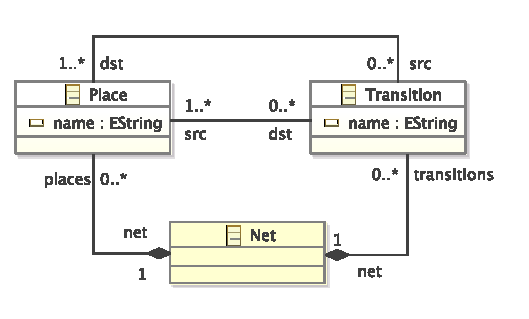
\includegraphics[scale=0.75]{petri_nets_step0.pdf}
  \caption{Original Petri nets metamodel.}
  \label{fig:original_mm}
\end{figure}

The evolved metamodel is shown in Figure~\ref{fig:evolved_mm}. \texttt{Place}s are connected to \texttt{Transition}s via instances of \texttt{PTArc}. Likewise, \texttt{Transition}s are connected to \texttt{Place}s via \texttt{TPArc}. Both \texttt{PTArc} and \texttt{TPArc} inherit from \texttt{Arc}, and therefore can be used to specify a \texttt{weight}.

\begin{figure}[htbp]
  \centering
  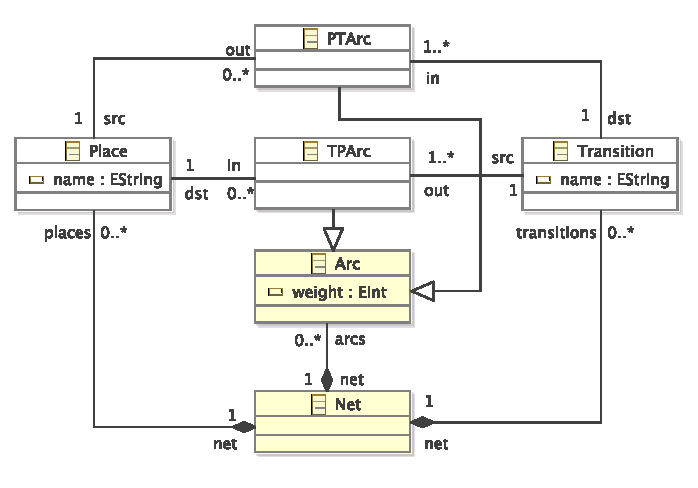
\includegraphics[scale=0.75]{petri_nets_step1.pdf}
  \caption{Evolved Petri nets metamodel.}
  \label{fig:evolved_mm}
\end{figure}

Models that were consistent with the original metamodel may not be consistent with the evolved metamodel. For example, \texttt{Transition} objects can no longer define values for \texttt{src} and \texttt{dst} features, and must define at least one value for the \texttt{in} and \texttt{out} features.

The migration strategy for this evolution varies when specified in ATL, Groovy-for-COPE and Flock, largely due to the differences in the way in which each approach initialises migrated models. When specified in ATL, migration must copy values from original to migrated model, as shown on lines 5-6, 12 and 20 of Listing~\ref{lst:quantitive_etl}. When using Groovy-for-COPE, values contained in slots that no longer correspond to features in the migrated metamodel must be unset, as shown on lines 2, 9 and 18-19 of Listing~\ref{lst:quantitive_cope}. Finally, Flock initialises the migrated model by copying values only for those features that remain unchanged in the migrated model. Consequently, no explicit copying or unsetting is required in Listing~\ref{lst:quantitive_flock}; the migration strategy manipulates only metafeatures that do not exist in the evolved metamodel (\texttt{Transition\#src} and \texttt{Transition\#dst}) and the new metaclasses, \texttt{TPArc} and \texttt{PTArc}.

\begin{lstlisting}[basicstyle=\ttfamily\footnotesize, flexiblecolumns=true, numbers=left, nolol=true, caption=Petri nets model migration in ATL, label=lst:quantitive_etl, language=ETL, tabsize=2]
rule Nets {
	from
		o : Before!Net
	to
	  m : After!Net ( places <- o.places, transitions <- o.transitions )
}

rule Places {
	from
		o : Before!Place
	to
		m : After!Place ( name <- o.name )
}

rule Transitions {
	from
		o : Before!Transition
	to
		m : After!Transition (
			name <- o.name,
			"in" <- o.src->collect(p | thisModule.PTArcs(p,o)),
			out  <- o.dst->collect(p | thisModule.TPArcs(o,p))
		)
}

lazy rule PTArcs {
	from
		place       : Before!Place,
		destination : Before!Transition
	to
		ptarcs : After!PTArc (
			src <- place,
			dst <- destination,
			net <- destination.net
		)
}

lazy rule TPArcs {
	from
		transition  : Before!Transition,
		destination : Before!Place
	to
		tparcs : After!TPArc (
			src <- transition,
			dst <- destination,
			net <- transition.net
		)
}
\end{lstlisting}


\begin{lstlisting}[basicstyle=\ttfamily\footnotesize, flexiblecolumns=true, numbers=left, nolol=true, caption=Petri nets model migration in COPE, label=lst:quantitive_cope, language=Java, tabsize=2]
for (transition in Transition.allInstances) {
  for (source in transition.unset('src')) {
    def arc = petrinets.PTArc.newInstance()
    arc.src = source
    arc.dst = transition
    arc.net = transition.net
  }

  for (destination in transition.unset('dst')) {
    def arc = petrinets.TPArc.newInstance() 
    arc.src = transition
    arc.dst = destination
    arc.net = transition.net
  }
}

for (place in Place.allInstances) {
  place.unset('src')
  place.unset('dst')
}
\end{lstlisting}


\begin{lstlisting}[basicstyle=\ttfamily\footnotesize, flexiblecolumns=true, numbers=left, nolol=true, caption=Petri nets model migration in Flock, label=lst:quantitive_flock, language=Flock, tabsize=2]
migrate Transition {
  for (source in original.src) {
    var arc := new Migrated!PTArc;
    arc.src := source.equivalent();
    arc.dst := migrated;
    arc.net := original.net.equivalent();
  }

  for (destination in original.dst) {
    var arc := new Migrated!TPArc;
    arc.src := migrated;
    arc.dst := destination.equivalent();
    arc.net := original.net.equivalent();
  }
}
\end{lstlisting}

With regard to the way in which they initialise the migrated model, COPE and ATL are opposites. The former initialises an exact copy of the original model, and so unset operations must be used when the value of a feature should not have been copied. By contrast, the latter initialises an empty model, and so explicit assignment operations must be used to copy values from original to migrated model for each feature that is not affected by the metamodel evolution.

This difference explains the results shown in Table~\ref{tab:model_operations_results}. Firstly, because Flock requires no unsetting of affected model elements nor explicit copying of unaffected model elements, less model operations are used when specifying a migration strategy with Flock than is used when specifying the same migration strategy with Groovy-for-COPE or with ATL. Secondly, there are more features unaffected by metamodel evolution than affected. Consequently, specifying model migration with ATL for the examples shown in Table~\ref{tab:model_operations_results} requires more model operations than in Groovy-for-COPE.


\paragrah{Side-Effects during Initialisation}
The measurements observed for one of the examples of co-evolution from Chapter~\ref{Analysis}, Change Reference to Containment, cannot be explained by the difference in copying strategy. Instead, the way in which models are initialised by the migration languages must be considered. When a reference feature is changed to a containment reference during metamodel evolution, constructing the migrated model by starting from the original model (as is the case with Groovy-for-COPE and, when the feature is not renamed, also Flock) can have side-effects which complicate migration.

In the Change Reference to Containment example, a \texttt{System} initially comprises \texttt{Port}s and \texttt{Signature}s (Figure~\ref{fig:ref2cont_original_mm}). A \texttt{Signature} references any number of \texttt{ports}. The metamodel is to be evolved so that \texttt{Port}s can no longer be shared between \texttt{Signature}s.

\begin{figure}[htbp]
  \centering
  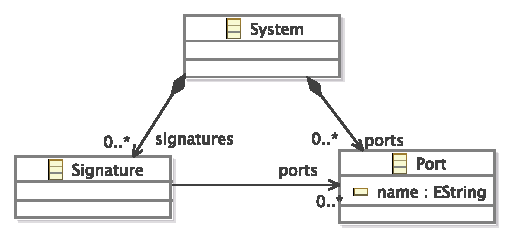
\includegraphics[scale=0.75]{change_ref_to_cont_before.pdf}
  \caption{Original metamodel.}
  \label{fig:ref2cont_original_mm}
\end{figure}

The evolved metamodel is shown in Figure~\ref{fig:ref2cont_evolved_mm}. \texttt{Signature}s now contain - rather than reference - \texttt{Port}s. Consequently, the \texttt{ports} feature of \texttt{System} is no longer required and is removed.

\begin{figure}[htbp]
  \centering
  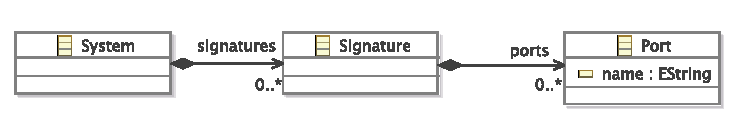
\includegraphics[scale=0.75]{change_ref_to_cont_after.pdf}
  \caption{Evolved metamodel.}
  \label{fig:ref2cont_evolved_mm}
\end{figure}

The migration strategy is straightforward in ATL: for each \texttt{Signature} in the original model, each member of the \texttt{ports} feature is cloned, using a lazy rule, and added to the \texttt{ports} feature of the equivalent \texttt{Signature}.

\begin{lstlisting}[basicstyle=\ttfamily\footnotesize, flexiblecolumns=true, numbers=left, nolol=true, caption=Change R to C model migration in ATL, label=lst:ref2cont_atl, language=ATL, tabsize=2]
rule Systems {
	from
		o : Before!System
	to
		m : After!System ( signatures <- o.signatures )
}

rule Signature {
	from
		o : Before!Signature
	to
		m : After!Signature (
			ports <- o.ports->collect(p | thisModule.Port(p))
		)
}

lazy rule Port {
	from
		o : Before!Port
	to
		m : After!Port ( name <- o.name )
\end{lstlisting}

In Flock and Groovy-for-COPE, migration is less straightforward because, during migration, the value of a containment reference (\texttt{Signature\#ports}) is set automatically by the migration strategy execution engine. When a containment reference is set, the contained objects are removed from their previous containment reference (i.e. setting a containment reference can have side-effects). Therefore, in a \texttt{System} where more than one \texttt{Signature} references the same \texttt{Port}, the migrated model cannot be formed by copying the contents of \texttt{Signature\#ports} from the original model. Attempting to do so causes each \texttt{Port} to be contained only in the last referencing \texttt{Signature} that was copied.

In Groovy-for-COPE, the containment nature of the reference is not enforced until after the migration strategy is executed. Hence, the migration strategy can be specified by unsetting the contents of the \texttt{ports} reference (line 4 of Listing~\ref{lst:ref2cont_cope}), and creating a copy of each referenced \texttt{Port} (lines 5-7 of Listing~\ref{lst:ref2cont_cope}). Unlike the ATL migration strategy, the ports in the Groovy-for-COPE migration strategy are cloned in the same model as the original port. Consequently, the Groovy-for-COPE migration strategy must either only clone ports that are referenced by more than one signature or clone every referenced port, but delete all of the original ports. The latter approach requires 2 more model operations (to populate and delete the original ports) than the former (shown in Listing~\ref{lst:ref2cont_cope}).

\begin{lstlisting}[basicstyle=\ttfamily\footnotesize, flexiblecolumns=true, numbers=left, nolol=true, caption=Change R to C model migration in COPE, label=lst:ref2cont_cope, language=COPE, tabsize=2]
def contained = []

for(signature in refactorings_changeRefToCont.Signature.allInstances) {
  for(port in signature.ports)) {
	  // when more than one Signature references this port
	  if (contained.contains(port)) {
      def clone = Port.newInstance()
      clone.name = port.name
      signature.ports.add(clone)
      signature.ports.remove(port)
		} else {
			contained.add(port)
		}
  }
}

for(port in refactorings_changeRefToCont.Port.allInstances) {
	if (not refactorings_changeRefToCont.Signature.allInstances.any { it.ports.contains(port) }) {
	  	port.delete()
	}
}
\end{lstlisting}

In Flock, the containment nature of the reference is enforced when the migrated model is initialised. Because changing the contents of a containment reference can have side-effects, a \texttt{Port} that appears in the \texttt{ports} reference of a \texttt{Signature} in the original model may not have been automatically copied to the \texttt{ports} reference of the equivalent \texttt{Signature} in the migrated model during initialisation. Consequently, the migration strategy must check the \texttt{ports} reference of each migrated \texttt{Signature}, cloning only those \texttt{Port}s that have not be automatically copied during initialisation (see line 3 of Listing~\ref{lst:ref2cont_flock}).

\begin{lstlisting}[basicstyle=\ttfamily\footnotesize, flexiblecolumns=true, numbers=left, nolol=true, caption=Change R to C model migration in Flock, label=lst:ref2cont_flock, language=Flock, tabsize=2]
migrate Signature {
	for (port in original.ports) {
		if (migrated.ports.excludes(port.equivalent())) {
			var clone := new Migrated!Port;
			clone.name := port.name;
			migrated.ports.add(clone);
		}
	}
}

delete Port when: not Original!Signature.all.exists(s|s.ports.includes(original))
\end{lstlisting}


The Groovy-for-COPE and Flock migration strategies must also remove any \texttt{Port}s which are not referenced by any \texttt{Signature} (lines 17-21 of Listing~\ref{lst:ref2cont_cope}, and line 11 of Listing~\ref{lst:ref2cont_flock} respectively), whereas the ATL migration strategy, which initialises any empty migrated model, does not copy unreferenced \texttt{Port}s.

When a non-containment reference is changed to a containment reference, a Flock migration strategy requires one more more model operation than the equivalent ATL migration strategy: to delete model elements that are not contained in any instance of the containment reference (line 11 of Listing~\ref{lst:ref2cont_flock}). A Groovy-for-COPE migration strategy requires three more model operations than the equivalent ATL migration strategy: one to delete model elements that are not contained in any instance of the containment reference (lines 17-21 of Listing~\ref{lst:ref2cont_cope}), one to dereference model elements that have already been cloned (line 10 of Listing~\ref{lst:ref2cont_cope}), and one to mark a model element as contained (line 12 of Listing~\ref{lst:ref2cont_cope}).  In the example considered here, the ATL migration strategy requires one more model operation than the Flock and Groovy-for-COPE migration strategies (to copy the contents of System\#signature features from original to migrated model), due to the difference in copying strategy. This leads to the result shown in Table~\ref{tab:model_operations_results}: the Flock and ATL migration strategies have an equal number of model operations, while the COPE migration strategy has two more.


\subsubsection{Summary}
This section has compared the model migration languages

- Make clear the contribution: no other research has attempted to compare model migration languages. It's not clear how it should be done. This is a start. 
- Not trying to argue that the figures are statistically significant. Just an approximation of what we're trying to measure.
- Extensions: measure cyclomatic complexity, etc
